\documentclass[9pt,twocolumn,twoside]{gsajnl_modified}
% Use the documentclass option 'lineno' to view line numbers

\articletype{inv} 

\title{Recovery of a deleted deep sequencing data set sheds new light on the early spread of SARS-CoV-2 in Wuhan}

\author[]{\Large Jesse D. Bloom}

\affil[]{Fred Hutchinson Cancer Research Center}
\affil[]{Howard Hughes Medical Institute}
\affil[]{Seattle, WA, USA}

\keywords{}

\runningtitle{} % For use in the footer 
\runningauthor{}

\begin{abstract}
Abstract here
\end{abstract}

\begin{document}

\maketitle
\thispagestyle{firststyle}
%\marginmark
\firstpagefootnote

\correspondingauthoraffiliation{}{Corresponding author: \href{mailto:jbloom@fredhutch.org}{jbloom@fredhutch.org}}
\vspace{-33pt}% Only used for adjusting extra space in the left column of the first page

\lettrine[lines=2]{\color{color2}T}{}he origins... 

\section{Results}

\subsection{Identification of a SARS-CoV-2 deep sequencing data set that has been removed from the NCBI's Sequence Read Archive}
During the course of my research, I read a paper by \citet{farkas2020insights} that analyzed SARS-CoV-2 deep sequencing data from the Sequence Read Archive (SRA), which is a repository maintained by the NIH's National Center for Biotechnology Information (NCBI).
The first supplementary table of \citet{farkas2020insights} lists all SARS-CoV-2 deep sequencing data sets available from the SRA as of March 30, 2020.
I have digitally archived a copy of this table in the Wayback Machine at \url{https://web.archive.org/web/20210502130356/https://dfzljdn9uc3pi.cloudfront.net/2020/9255/1/Supplementary_Table_1.xlsx}. 

Half the entries in this table refer to a deep sequencing project (BioProject PRJNA612766) by Wuhan University that is described in the table as Oxford Nanopore sequencing of SARS-CoV-2 amplicons.
The table indicates this project contains 141 SRA accessions, each corresponding to a different sequencing run.
Because I had never encountered any other mention of this sequencing project, I performed a Google search for ``PRJNA612766,'' and found no search hits other than the supplementary table itself.
Searching for ``PRJNA612766'' in the NCBI's SRA search box returned a message of ``No items found.''

I then searched for individual sequencing run accessions in the NCBI's SRA search box.
These searches returned messages indicating that sequencing runs had been removed (Figure~\ref{fig:acc_removed}).

\begin{figure}[]
\centering
\fbox{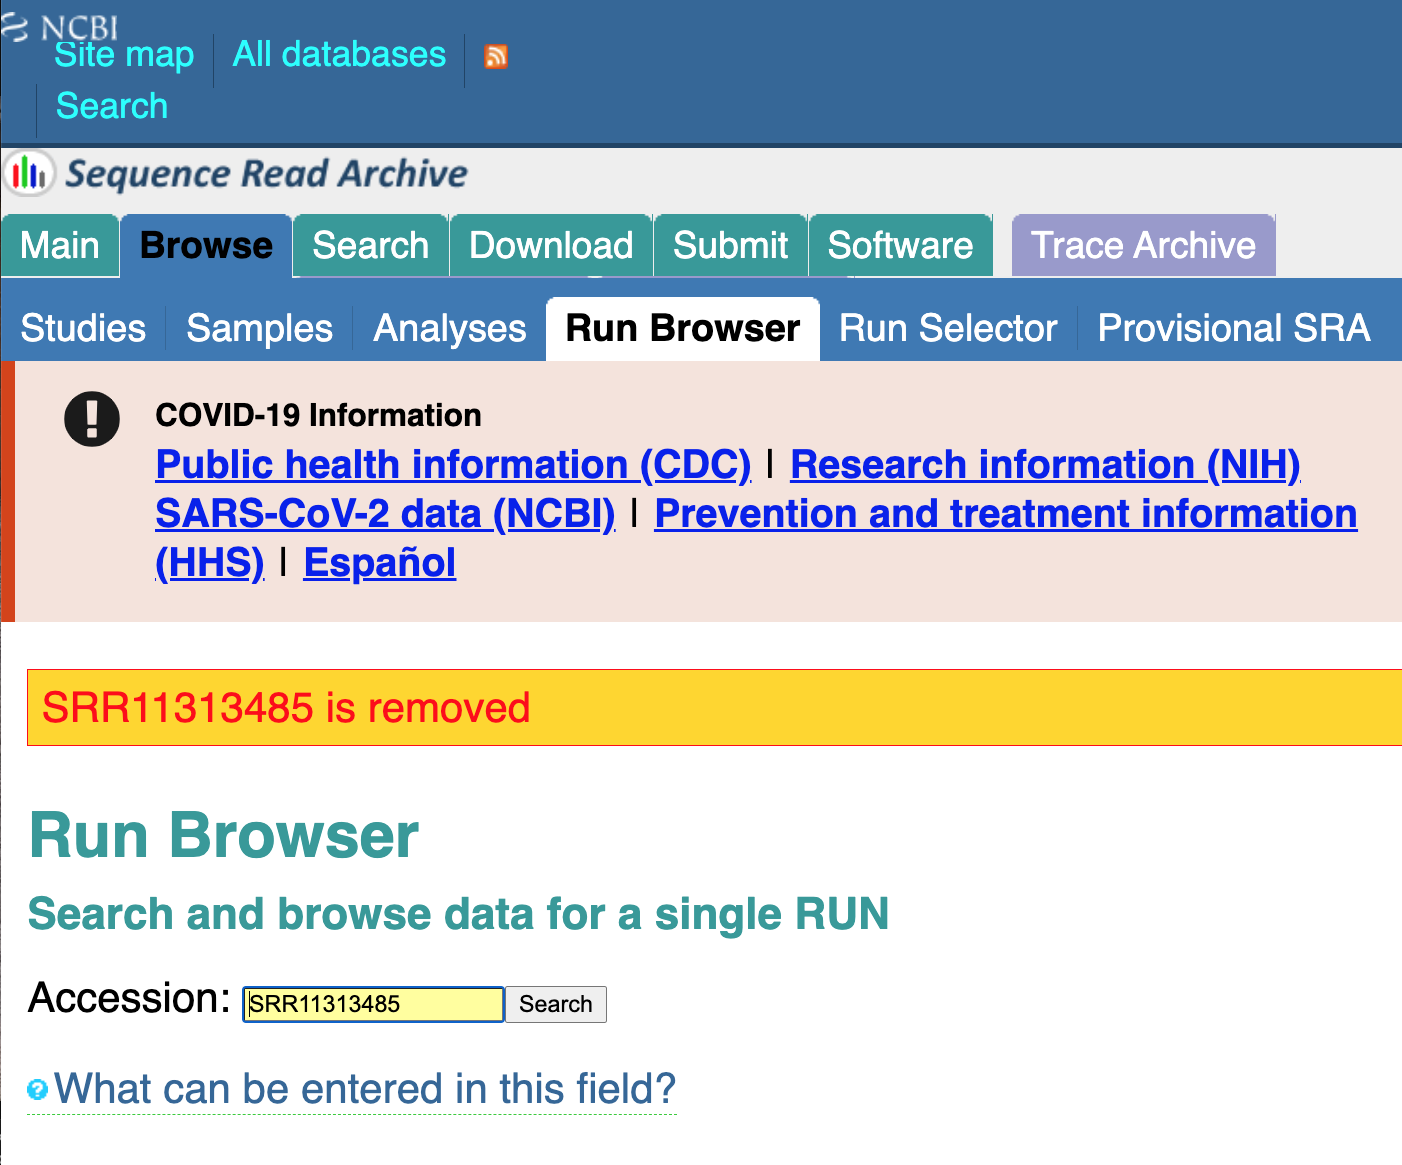
\includegraphics[trim={0.2in 0 0 9in},clip,width=\linewidth]{figures/acc_removed.png}}
\caption{Accessions from deep sequencing project PRJNA612766 have been removed from the SRA.
Shown is the result of searching for ``SRR11313485'' to reach the \url{https://trace.ncbi.nlm.nih.gov/Traces/sra/?run=SRR11313485}.
A copy of this result has been digitally archived on the Wayback Machine at \url{https://web.archive.org/web/20210502131630/https://trace.ncbi.nlm.nih.gov/Traces/sra/?run=SRR11313485}.
}%
\label{fig:acc_removed}
\end{figure}

The SRA is designed to serve as a permanent archive of deep sequencing data.
The SRA documentation states that after a sequencing run is uploaded, ``neither its files can be replaced nor filenames can be changed,'' and that data can only be deleted by directly e-mailing SRA staff with the reason for requesting the deletion~\citep{SRA_deletion}.
An example of this process from another study is in Figure~\ref{fig:pangolin_emails}, which shows e-mails between NCBI staff and the lead author of a paper on pangolin coronaviruses~\citep{xiao2020isolation} to which the journal \textit{Nature} added an editor's note on November 11, 2020, due to concerns about the identity of the underlying samples~\citep{chan2020single}.

\begin{figure}[]
\centering
\fbox{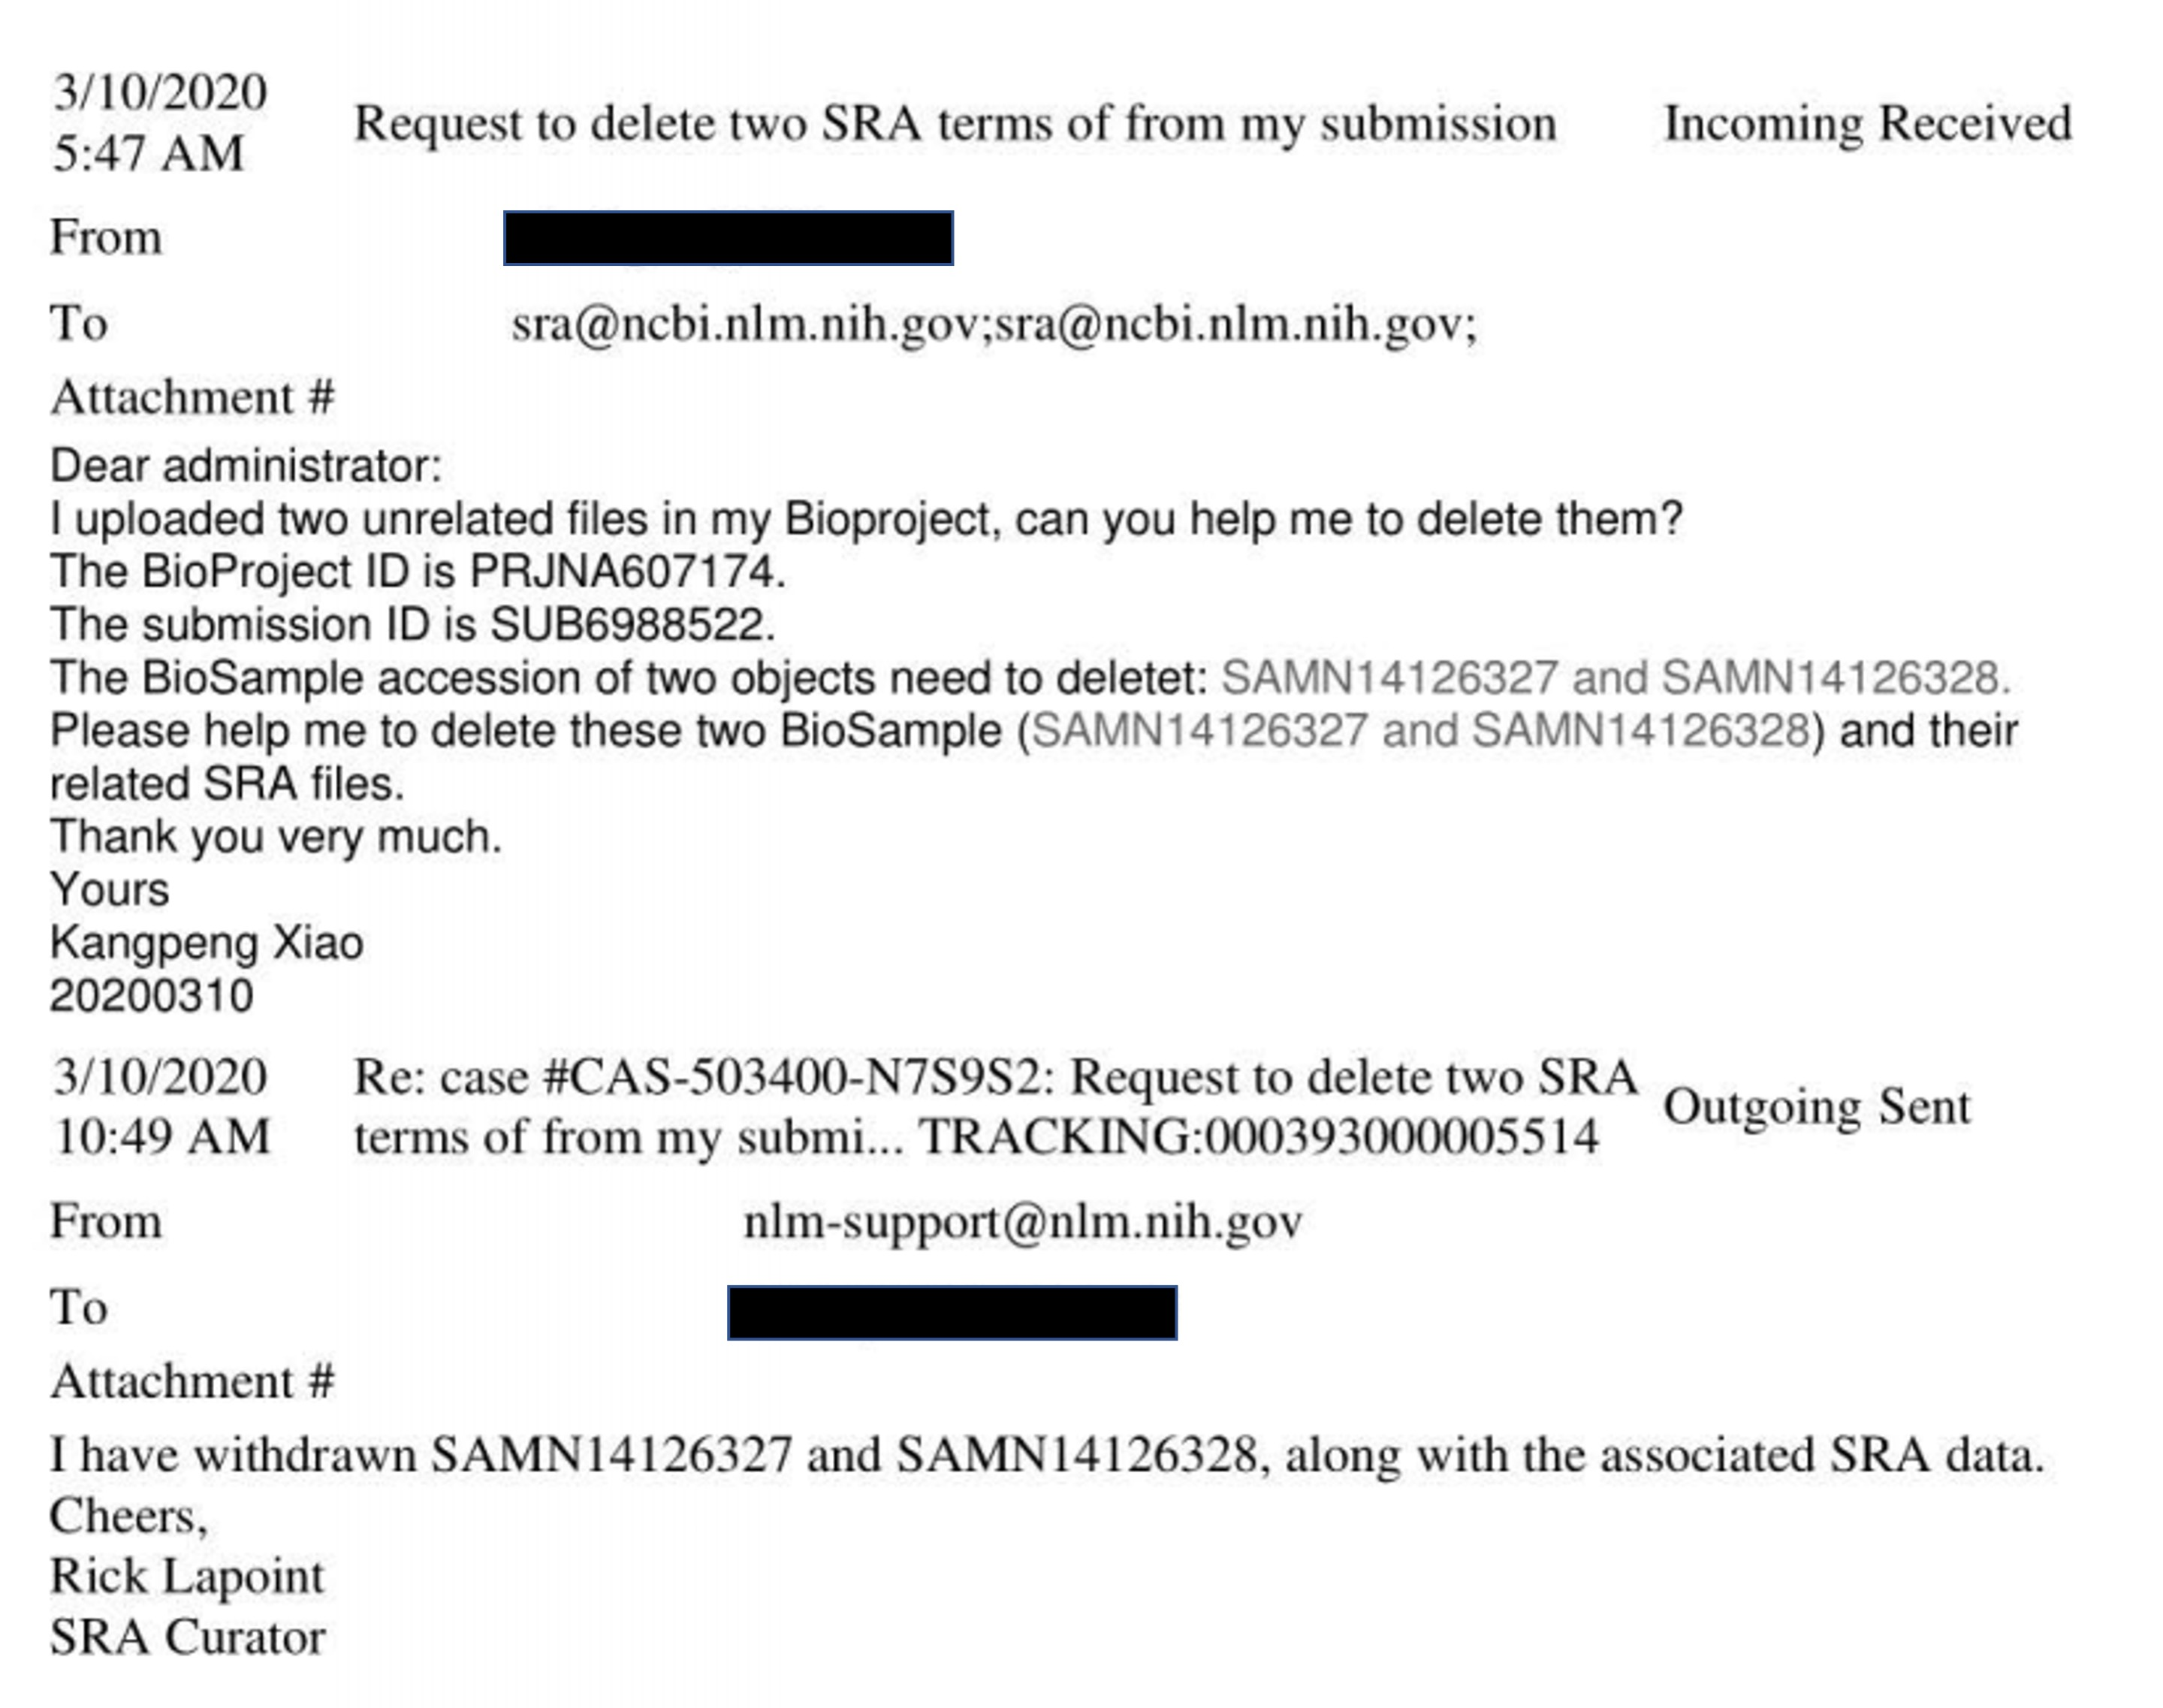
\includegraphics[trim={0.8in 0.8in 1.1in 1in},clip,width=\linewidth]{figures/pangolin_emails.jpg}}
\caption{Example of the process to delete SRA data.
The image shows an excerpt of e-mails between the lead author of the pangolin coronavirus paper \citet{xiao2020isolation} and SRA staff.
The full e-mails are at \url{https://usrtk.org/wp-content/uploads/2020/12/NCBI-Emails.pdf}.
}
\label{fig:pangolin_emails}
\end{figure}

Taken together, these facts indicate that subsequent to March 30, 2020, someone must have e-mailed the NCBI to reques deletion of the SARS-CoV-2 deep sequencing project PRJNA612766.

\subsection{The deleted data set contains sequencing of viral samples collected early in the Wuhan outbreak}
The metadata in the first supplementary table of \citet{farkas2020insights} indicates that the samples in the deleted project PRNJA612766 were collected by Aisu Fu and Renmin Hospital of Wuhan University.
Google searching for these terms revealed the samples were related to a study posted as pre-print on \textit{medRxiv} in early March of 2020~\citep{Wang2020medRxiv}, and subsequently published in the journal \textit{Small} in June of 2020~\citep{Wang2020small}.

The study describes an approach to diagnose infection with SARS-CoV-2 and other respiratory viruses by Oxford Nanopore sequencing.
This approach involved reverse-transcription of total RNA from swab samples, followed by PCR with specific primers that generated amplicons covering portions of the viral genome.
These amplicons were then sequenced on an Oxford Nanopore GridION, and infection with SARS-CoV-2 was diagnosed if the resulting sequencing yielded a sufficiently large number of reads aligning to the SARS-CoV-2 genome.
Importantly, the study notes that this approach yields genetic information about the sequence of the virus as well enabling diagnosis of infection.

The pre-print~\citep{Wang2020medRxiv} says the approach was applied to ``45 nasopharyngeal swab samples from outpatients with suspected COVID-19 early in the epidemic.''
The digital object identifier (DOI) for the pre-print indicates that it was processed by \textit{medRxiv} on March 4, 2020, which is one day after China's State Council ordered that all papers related to COVID-19 must be approved by a centralized group to ensure that scientific publications were coordinated ``like moves in a game of chess''~\citep{Kang2020}.
The final published manuscript~\citep{Wang2020small} updated the description of these 45 samples to say that they were obtained ``early in the epidemic (January 2020).''
Both the pre-print and published manuscript say that 34 of the 45 early epidemic samples were positive in the sequencing-based diagnostic approach.
In addition, they both state that the approach was then later applied to 16 additional samples collected on February 11 and 12 of 2020 from SARS-CoV-2 patients hospitalized at Renmin Hospital of Wuhan University.

There is complete concordance between the deep sequencing accessions for project PRJNA612766 in the supplementary table of \citet{farkas2020insights} and the biological samples described by \citet{Wang2020medRxiv}.
Specifically, there are 89 sequencing accessions corresponding to the 45 early epidemic samples, with these samples named like wells in a 96-well plate (A1, A2, etc).
The number of accessions is approximately twice the number of early epidemic samples because each sample has data for two nanopore sequencing runtimes except one sample (B5) with just one runtime.
 There are 31 sequencing accessions corresponding to the 16 samples collected in February from Renmin Hospital patients, with these samples named R01, R02, etc.
 Again, the number of accessions is approximately twice the number of samples because all but one sample (R04) has data for two different sequencing runtimes.
 In addition, there are 7 accessions corresponding to positive and negative controls, 2 accessions corresponding to other respiratory virus samples, and 112 samples corresponding to plasmids used for the initial benchmarking and development of the approach.
 Together, these samples and controls account for all 241 accessions listed for PRJNA612766 in the supplementary table of \citet{farkas2020insights}.

Neither the pre-print~\citep{Wang2020medRxiv} or published manuscript~\citep{Wang2020small} contain any corrections or notes that indicate a scientific reason for deleting the study's sequencing data from the SRA.

\subsection{Recovery of the deleted sequencing data from the Google cloud} 



\bibliography{references}

\end{document}
